\documentclass[11pt, oneside]{article}   	% use "amsart" instead of "article" for AMSLaTeX format
\usepackage{geometry}                		% See geometry.pdf to learn the layout options. There are lots.
\geometry{letterpaper}                   		% ... or a4paper or a5paper or ... 
%\geometry{landscape}                		% Activate for for rotated page geometry
%\usepackage[parfill]{parskip}    		% Activate to begin paragraphs with an empty line rather than an indent
\usepackage{graphicx}				% Use pdf, png, jpg, or eps� with pdflatex; use eps in DVI mode
								% TeX will automatically convert eps --> pdf in pdflatex		
\usepackage{amssymb}
\usepackage{amsmath}
\usepackage{parskip}
\usepackage{color}
\usepackage{hyperref}

\title{Elementary complex functions}
%\author{The Author}
%\section{}
%\subsection*{}
\date{}							% Activate to display a given date or no date

\graphicspath{{/Users/telliott_admin/Dropbox/Tex/png/}}
% \begin{center} 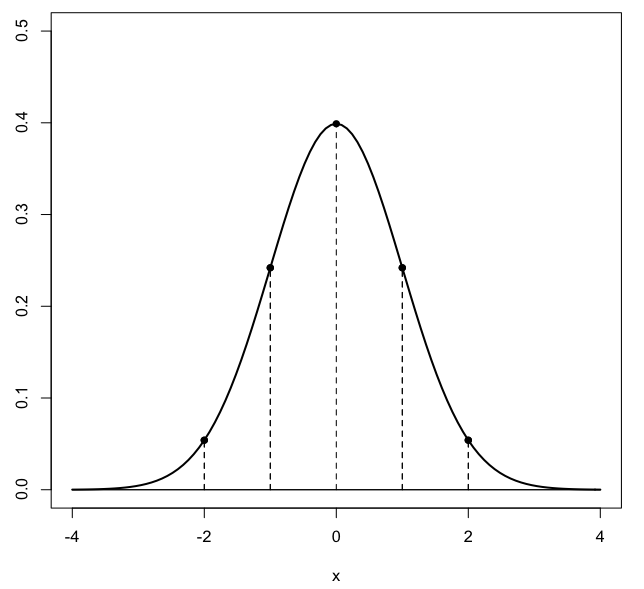
\includegraphics [scale=0.4] {gauss3.png} \end{center}
\begin{document}
\maketitle
\Large

First of all, write
\[ e^z = e^{x + iy} \]
\[ = e^x e^{iy} \]
We can thus visualize the complex exponential as having modulus $e^x$ and argument $y$.

Reversing Euler:
\[ = e^x (\cos y + i \sin y) \]
\[ = e^x \cos y + i e^x \sin y \]

So the real part of $e^z$ is 
\[ u(x,y) = e^x \cos y \]
\[ u_x = e^x \cos y \]
\[ u_y = - e^x \sin y \]
and the imaginary part is
\[ v(x,y) = e^x \sin y \]
\[ v_x = e^x \sin y \]
\[ v_y = e^x \cos y \]
Hence
\[ u_x = v_y \]
\[ u_y = - v_x \]
The CRE conditions are satisfied and the complex exponential $e^z$ is analytic.  (Which, according to Shankar, we could have predicted, since it depends only on $z$ and not on $z*$).

Notice also that (evaluating the derivative along $\Delta y =0$:
\[ f'(z) = u_x + iv_x  \]
\[ = e^x \cos y + i e^x \sin y = z \]
The exponential is its own derivative.

Which is good because we want our definitions for the complex functions to give the standard results when $z$ has only a real part, i.e. when $y=0$.

Now, once more we recall Euler's formula (for a real variable $\theta$ or $x$):
\[ e^{i \theta} = \cos \theta + i \sin \theta \]
\[ e^{i x} = \cos x + i \sin x \]
Substitute $-x$ for $x$:
\[ e^{-i x} = \cos -x + i \sin -x \]
\[ = \cos x - i \sin x \]
By addition and subtraction we obtain:
\[ 2 \cos x = e^{i x} + e^{-i x} \]
\[ \cos x = \frac{e^{i x} + e^{-i x}}{2} \]
and
\[ 2i \sin x = e^{i x} - e^{-i x} \]
\[ \sin x = \frac{e^{i x} - e^{-i x}}{2i} \]

We will also need the hyperbolic sine and cosine later so let's just remind ourselves:
\[ 2 \cosh x = e^x + e^{-x} \]
\[ 2 \sinh x = e^x - e^{-x} \]

The derivative of the complex exponential is as we would hope and expect:
\[ \frac{d}{dz} e^z = e^z \]

This can be proved by using a Taylor series.  Shankar says to define $e^z$ in the same way as $e^x$.  That is:
\[ e^x = \sum_0^{\infty} \frac{x^n}{n!} \]
which we know converges because
\[ |x| < R = \lim_{n \rightarrow \infty} \frac{|a_n|}{|a_{n+1}|} \]
where $a_n = 1/n!$.  So
\[ e^z = \sum_0^{\infty} \frac{z^n}{n!} \]
and again we see that 
\[ \frac{d}{dz} \ e^z = e^z \]
differentiating the series term by term.

The complex exponential 
\[ e^z = e^x e^{iy} \]
has some properties that are not shared with the real exponential.  As we saw before, the angle $\theta + 2 \pi = \theta$ (and $2 \pi = 0$), so any number is really a family of numbers with different $\theta + 2 \pi k$ for integer $k$.

In particular, $e^z$ is periodic with a period of $2 \pi i$.  Additionally, it is possible for $e^z$ to be negative.  Consider that it is possible that
\[ e^z = -1 \]
as follows.  Let $z = 0 + i\pi$.  Then 
\[ e^x = e^0 = 1 \]
and
\[ e^{iy} = e^{i\pi} = -1 \]
So
\[ e^z = e^x e^{iy} = e^x(\cos y + i \sin y) = 1 (-1) = -1 \]
On the other hand, $e^z$ \emph{cannot be zero}.
\[ e^z = e^x \cos y + i e^x \sin y = e^x(\cos y + i \sin y) \]
For $x \in \mathbb{R}$, $e^x > 0$ so the only way this could be zero would be if we can find a $y$ such that $\sin y$ and $\cos y$ were both zero.  Since there is no such $y$, we conclude that $e^z$ cannot be equal to zero.

\end{document}  